\chapter{Diseño\label{sec:diseño}}

Este proyecto consiste en una ampliación y cambio de enfoque de otro proyecto llevado a cabo de manera simultánea por una alumna de la Universidad Politécnica de Madrid llamada Nerea Urrestarazu que a su vez se basa en el Kit de demostración de rendimiento del ADS1299 proporcionado por Texas Instrument.

\begin{figure} [H]
    \centering
    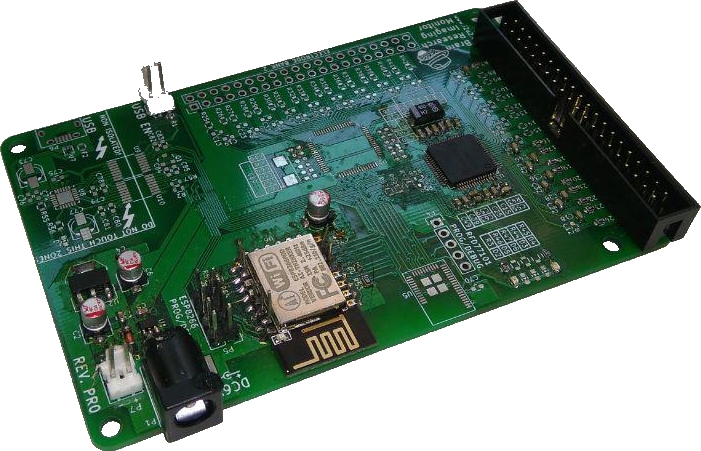
\includegraphics[width=7cm]{Placa_Nerea}
    \caption{Placa final del proyecto base}
    \label{fig:Placa_base}
\end{figure}

\section{Diseño base\label{sec:Diseno_base_N}}

El proyecto original trata sobre el diseño y desarrollo de una placa de adquisición de EEG haciendo uso de los integrados ADS1299 junto con un sistema de transmisión hacia el ordenador tanto inalámbricamente como a través de USB. La figura \ref{fig:Diseno_base} muestra las partes que componen dicho diseño.

\begin{figure} [H]
    \centering
    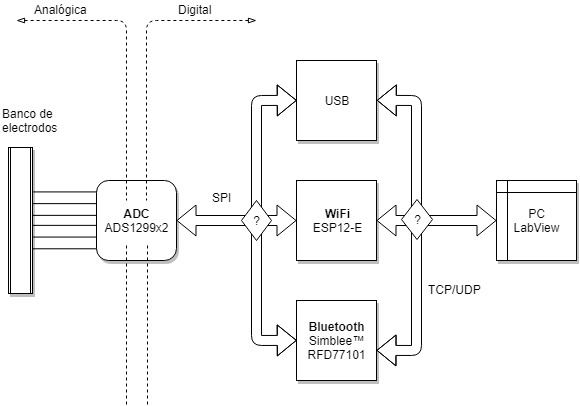
\includegraphics[width=7cm]{Esquema_diseno_base}
    \caption{Esquema del proyecto base}
    \label{fig:Diseno_base}
\end{figure}

\section{Adquisición de datos\label{sec:Adquisicion_N}}

La parte encargada de la adquisición está compuesta por un par de bancos de electrodos dispuestos en los laterales de la placa seguidos de un filtro paso-bajo con frecuencia de corte de 6.79Hz encargado de eliminar las componentes de frecuencias no deseadas. A continuación se encuentran conectados a sus respectivos bancos los convertidores Analógico-Digital ADS1299. 
\\Estos convertidores son capaces de adquirir información de forma independiente o en modo "Daisy Chain" y transmitirla a través de un puerto \gls{SPI} hacia otros dispositivos capaces de gestionarla.

\begin{figure} [H]
    \centering
    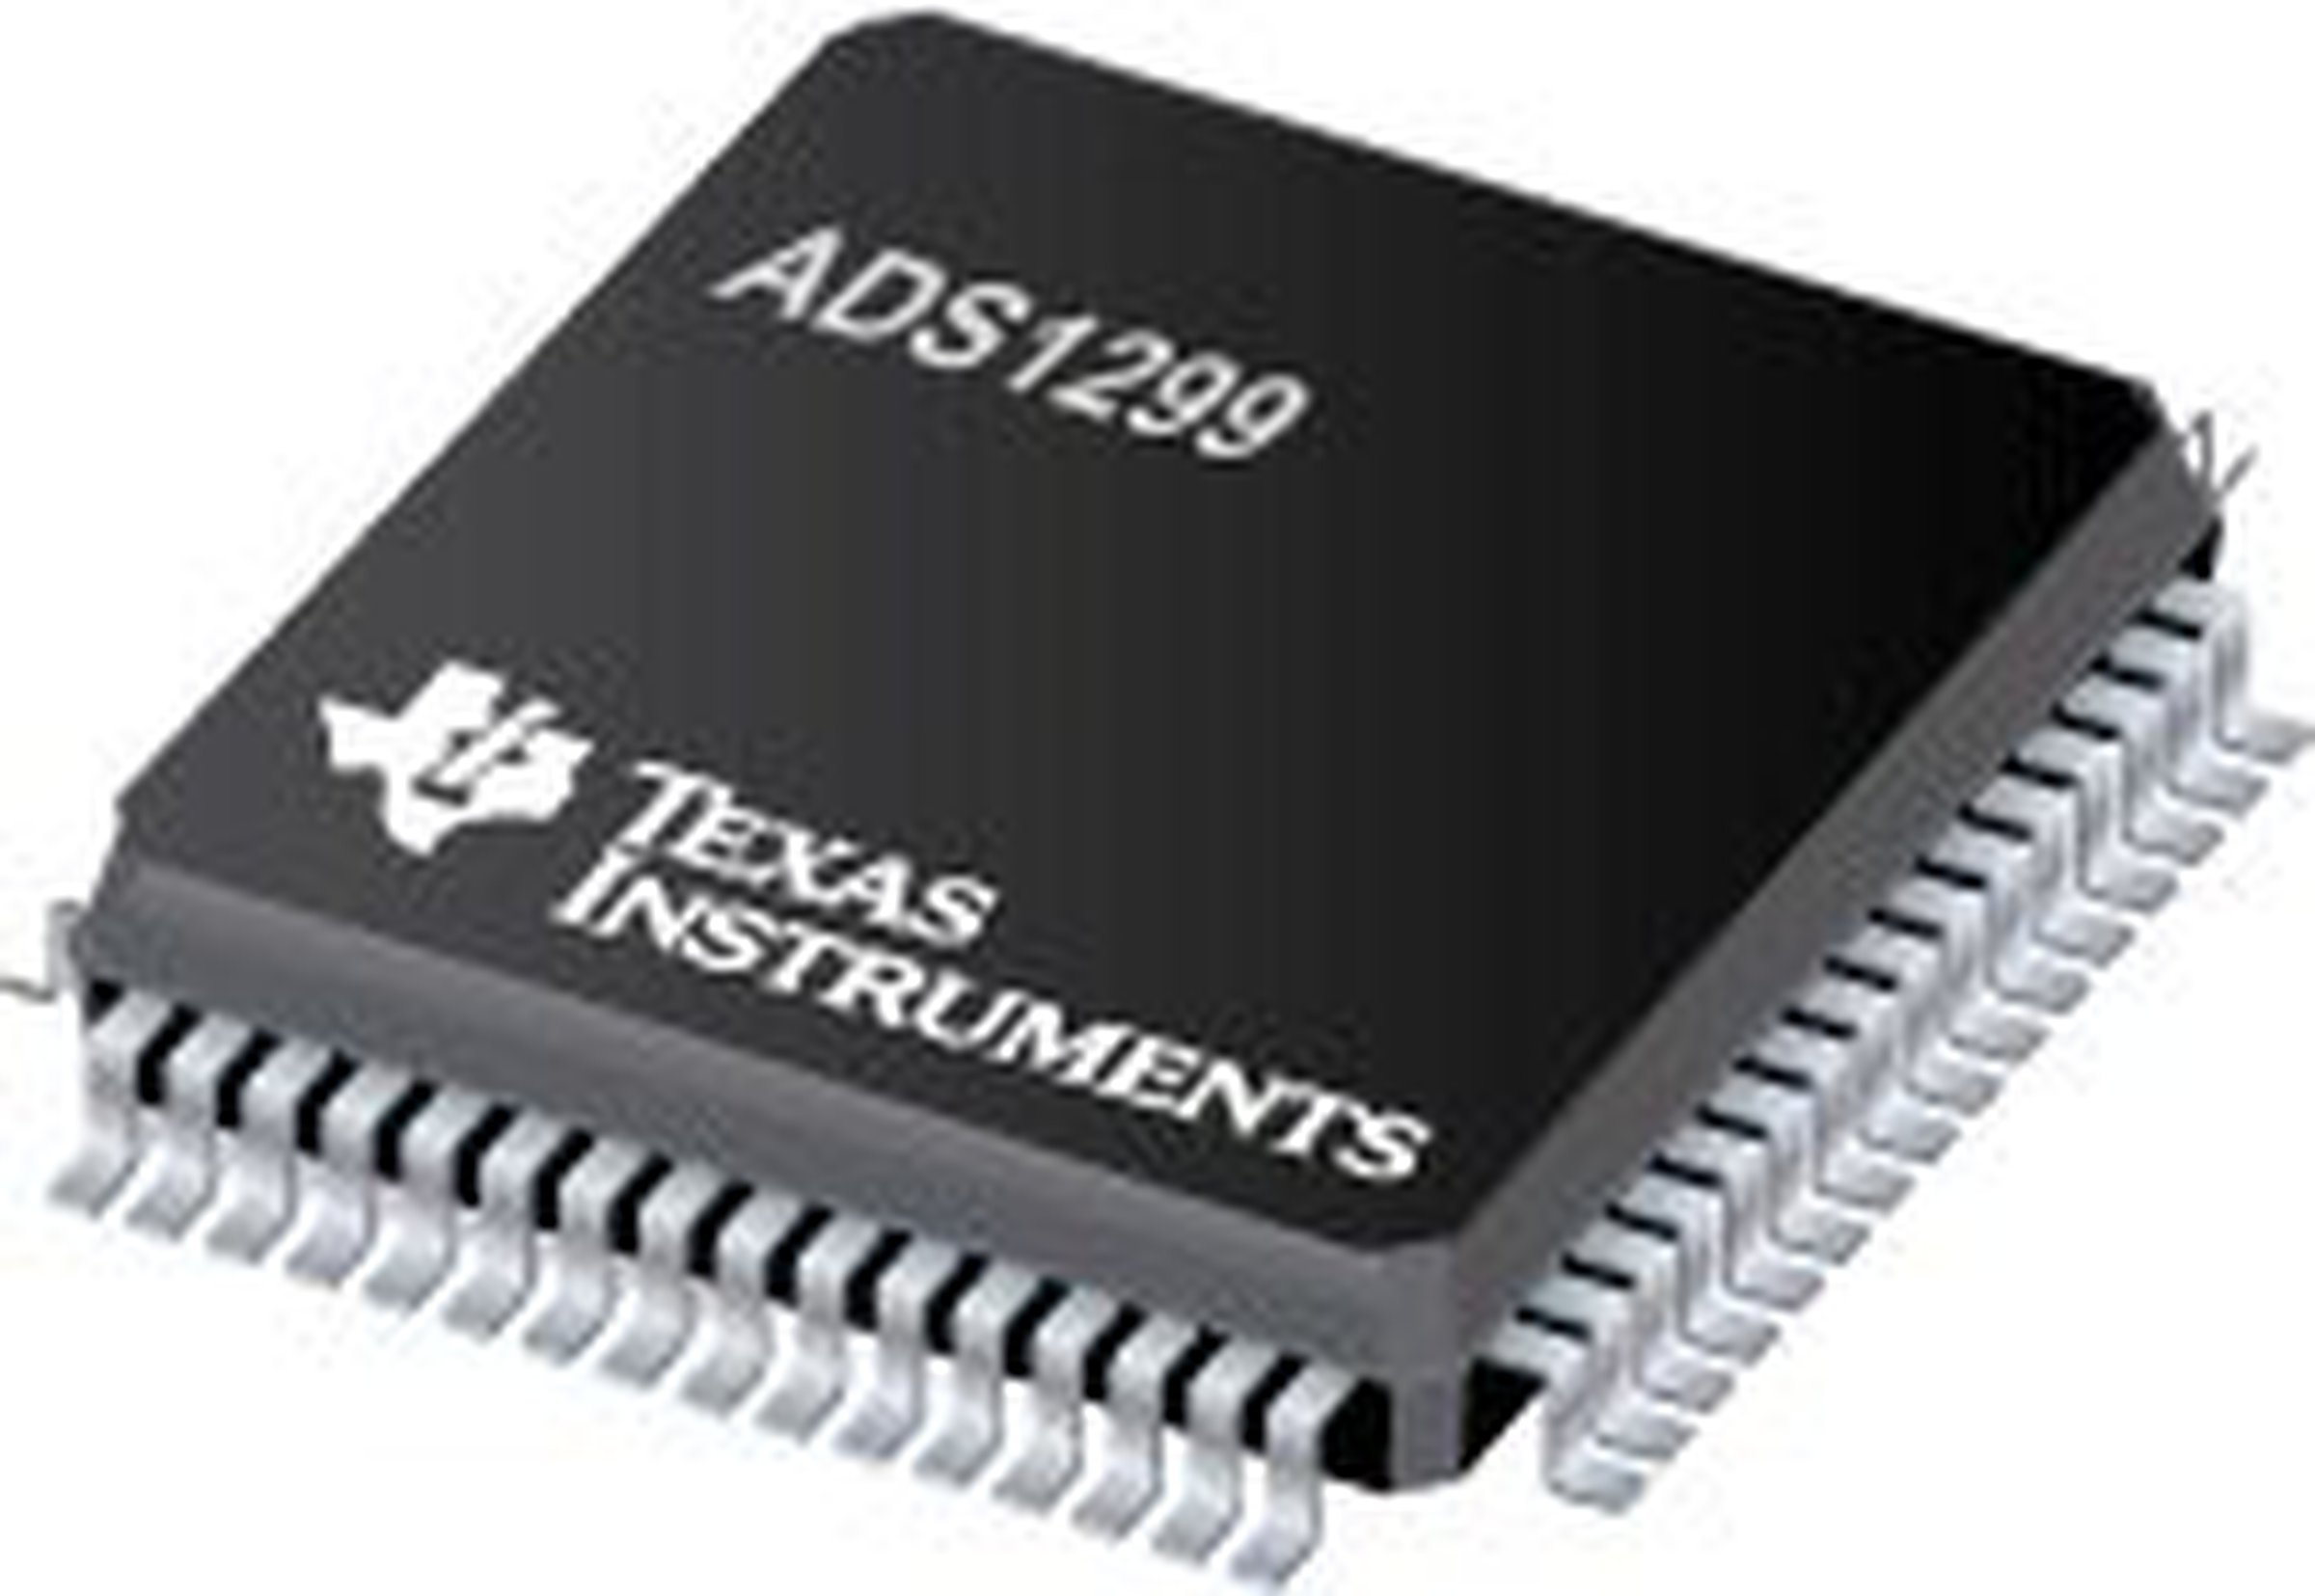
\includegraphics[width=7cm]{ADS1299}
    \caption{Convertidor Analógico-Digital ADS1299}
    \label{fig:ADS1299}
\end{figure}

\section{Transmisión de datos\label{sec:Transmisión_N}}

A continuación se encuentra la zona encargada de transmitir dicha información.
\\El transmisor hace uso de dos tecnologías distintas que funcionarán de forma excluyente seleccionables con un \textit{jumper}, a saber: WiFi o Bluetooth.

\subsection{WiFi\label{sec:WiFi_N}}

Para la transmisión de datos a través de WiFi se seleccionó el integrado ESP2866, también conocido como ESP12-E o nodemcu.
\\Este cuenta con un procesador 

\begin{figure} [H]
    \centering
    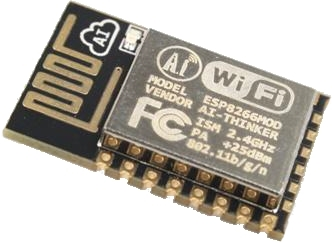
\includegraphics[width=7cm]{ESP8266}
    \caption{ESP8266}
    \label{fig:ESP8266}
\end{figure}

\subsection{Bluetooth\label{sec:Bluetooth_N}}



\subsection{USB\label{sec:USB_N}}


Hablar de la placa de Nerea y cómo la haces inteligente

Selección del STM

Diseño de la placa

	Comunicación con la otra placa (sandwich) vs Diseño de cero
	Alimentación
	Interfaces
